\documentclass[11pt,a4paper]{article}

\usepackage[T1]{fontenc}
\usepackage[utf8]{inputenc}
\usepackage[margin=1.1in]{geometry}
\usepackage{amsmath,amssymb,amsthm}
\usepackage[expansion=false]{microtype}
\usepackage{enumitem}
\usepackage{listings}
\usepackage{xcolor}
\usepackage{booktabs}
\usepackage{tikz}
\usetikzlibrary{calc,positioning}
\usepackage[hidelinks]{hyperref}

\tikzset{
  zxz/.style={circle, draw=black, fill=green!30, minimum size=5.5mm,
              inner sep=0.5pt, font=\scriptsize},
  zxx/.style={circle, draw=black, fill=red!30, minimum size=5.5mm,
              inner sep=0.5pt, font=\scriptsize},
  zxw/.style={thick},
  zxlab/.style={font=\scriptsize\itshape}
}

\lstset{
  basicstyle=\ttfamily\small,
  columns=fullflexible,
  keepspaces=true,
  frame=single,
  framesep=6pt,
  xleftmargin=12pt,
  xrightmargin=12pt,
  breaklines=true,
  captionpos=b
}

\theoremstyle{definition}
\newtheorem{definition}{Definition}[section]
\newtheorem{principle}[definition]{Principle}
\newtheorem{remark}[definition]{Remark}
\newtheorem{question}{Open Question}

\theoremstyle{plain}
\newtheorem{proposition}[definition]{Proposition}
\newtheorem{lemma}[definition]{Lemma}

\newcommand{\Meas}{\textsf{measure}}
\newcommand{\supp}{\operatorname{supp}}
\newcommand{\lbr}{[\![}
\newcommand{\rbr}{]\!]}
\newcommand{\gr}[1]{\lbr #1 \rbr}

\title{Measurement as a Move\\[4pt]
\large A quantum chess variant with bounded branching, adversarial collapse,\\
and a minimal observation language}

\author{L.~G. Meredith\\ \small F1R3FLY.io}

\date{September 2026}

\begin{document}

\maketitle

\begin{abstract}
We report the design of a quantum variant of chess in which a player may play a
superposition of at most $m$ classical moves, and may additionally elect, as a
whole turn, to force a measurement of the board. The literature contains two
mature lineages --- superposition of \emph{moves} in the possibilistic style of
Dorbec and Mhalla, and superposition of \emph{positions} under unitary dynamics
in the style of Cantwell --- but in every design we have found, measurement is
\emph{triggered} by a rule rather than \emph{elected} by a player. The elective
measurement move is the novel element, and it forces a series of further
choices which this note records: who resolves the measurement, what may be
asked, and what the branching bound counts. The design we arrive at resolves
the measurement adversarially (the opponent supplies the answer), which keeps
the game free of chance and answers the recent result of Scholten, Westerbaan
and Samardjiska that quantum moves confer no advantage against perfect
classical play. It equips the measurement move with a deliberately small
observation language whose atoms are patterns against the board and whose two
connectives are restricted so that one merges and one correlates, neither able
to impersonate the other. We give the grammar, the semantics, an optional phase
layer under which interference has the unusually legible reading of
\emph{menu deletion}, a sketch of the player as an f1r3lang process, and a list
of open questions, chief among them whether the branching bound is a
capability at all --- that is, whether the optimal $m$ for a perfect player
exceeds one. Three appendices work a nine-ply trace in the Italian Game in which
both players superpose both sides of a book fork, give a ZX-calculus semantics
for traces under which a trace compiles to one interferometer per Q-move that
closes, and verify the two against each other.
\end{abstract}

\tableofcontents

\section{Introduction}
\label{sec:intro}

The proposal under study is easy to state. A player may, on their turn, play a
\emph{superposition} of classical chess moves rather than a single one, subject
to a bound $m$ on how many moves may be superposed. A player may alternatively
spend their turn forcing a \emph{measurement}, collapsing some of the resulting
indeterminacy.

The first half of that proposal is well covered by existing work, twice over
and from two different directions. The second half appears to be unclaimed, and
it is where the design interest lies. In every quantum board game we have
located, measurement happens because a rule says it must: because a cycle of
entanglement has closed, because a capture has been attempted, because a stone
has been placed adjacent to a superposed stone. Nowhere is measurement a move a
player may choose to make, at a tempo cost, naming what is to be asked.

Making measurement elective turns out not to be a local addition. It interacts
with almost every other design choice, and pursuing those interactions is what
produced the design reported here. Section~\ref{sec:prior} reviews the prior
art and locates the gap precisely. Section~\ref{sec:axes} lays out the design
space as a set of independent axes. Section~\ref{sec:design} records the
choices we made and why. Sections~\ref{sec:obs} and~\ref{sec:moves} give the
observation and move languages, which are the two artefacts of the design most
likely to go wrong by accident and are therefore treated in detail.
Section~\ref{sec:sem} gives the semantics. Section~\ref{sec:phase} describes an
optional phase layer. Section~\ref{sec:f1r3lang} sketches the player as a
process in f1r3lang, connecting this variant to the multi-agent chess player
already under development. Section~\ref{sec:ladder} describes the branching
bound as a tournament structure. Section~\ref{sec:open} collects the open
questions.

A word on what kind of document this is. The design is not finished. Several
choices below are recorded as decided because they were decided in the course
of the dialogue that produced this note, and several others are recorded as
open because they turn on facts about the resulting game that only play or
search will supply. We have tried to be explicit about which is which.

\section{Prior art}
\label{sec:prior}

\subsection{Superposition of moves: the possibilistic lineage}

Dorbec and Mhalla's \emph{Toward Quantum Combinatorial Games}
\cite{dorbec2017} is the general form of the first half of our proposal. They
generalise Goff's quantum tic-tac-toe \cite{goff2006} to arbitrary
combinatorial games by allowing players to play superpositions of moves. In
their terminology a \emph{Q-move} is a set of classical moves; a \emph{run} is
a choice of one classical move from each Q-move played so far; and if a run
forms a legal sequence in the underlying classical game, the position it
reaches is a \emph{realisation}. They propose several rulesets, differing in
when superposed and unsuperposed moves may be played, and prove that the
rulesets separate: the same classical game can have different outcomes under
different rulesets. Their worked case is Nim.

Crucially, this lineage is \emph{possibilistic}. A superposition is a set of
realisations, carrying no amplitudes. There is no Born rule and no
interference. What quantum mechanics contributes is the branching structure and
the collapse discipline, not the linear algebra.

Burke, Ferland and Teng \cite{burke2020,burke2022} take up the framework,
concentrating on what they call flavour~D, in which classical moves are always
available as one-wide superpositions, so that the quantum game contains the
classical one. Their results are about complexity: starting from
superpositions, Nim becomes $\Sigma_2^p$-hard and Undirected Geography becomes
PSPACE-complete, and they exhibit abstract PSPACE-complete games whose quantum
extensions fall to each level of the polynomial hierarchy. They also make a
methodological observation that matters for us: in quantum combinatorial games
the \emph{description} of a move is part of the game definition, because move
description affects collapse. Two moves with the same effect on a classical
position may filter a superposition differently.

The same group's \emph{Transverse Wave} \cite{burke2021} and the recent
\emph{Cheqqers} \cite{cheqqers2025}, a quantum checkers built in flavour~D,
extend the lineage to further games.

\subsection{Superposition of positions: the unitary lineage}

Cantwell's Quantum Chess \cite{cantwell2019} is the serious engineering of the
other approach. The board is a quantum register, one qubit per square, and
moves are unitaries: split moves send a piece to two targets, merge moves
recombine, and the resulting dynamics exhibit superposition, entanglement and
interference. Measurement is present but is \emph{forced by move type} --- the
excluded and capture variants of each move require a measurement so that the
engine can unambiguously assign a piece to the target square. A measurement
rule additionally serves to keep the superposition small enough for the game to
remain tractable classically and comprehensible to a player.

Cantwell's treatment of the win condition is the one piece of his design we
adopt wholesale. There is no check; a player wins by capturing the opponent's
king with certainty, and while both kings have nonzero probability of being on
the board the game continues. Any design that admits a possibilistic notion of
check --- mate only if mated in every realisation --- makes superposition a
free escape from every mating net, and the game collapses.

\subsection{Other variants}

Akl's Quantum Chess \cite{akl2010} superposes piece \emph{identity} rather than
position: a piece is a superposition of types, and collapses to one of them
when touched. Goff's quantum tic-tac-toe \cite{goff2006} forces collapse when a
cycle of entanglement closes, and --- a detail we return to --- the player who
did \emph{not} create the cycle chooses where the collapse begins. Quantum Go
exists in several forms \cite{quantumgo2020}, with collapse triggered by
adjacency.

\subsection{The quantum Zermelo result}

Scholten, Westerbaan and Samardjiska \cite{scholten2026} give the result any
new design in this space must answer. Instantiating Zermelo's theorem in the
quantum setting, they show that quantum effects convey no advantage against a
classical player who plays a perfect classical strategy; the quantum player's
edge arises only from amplifying the classical player's mistakes.

The lesson we take is not that quantum variants are pointless, but that a
design which adds \emph{randomness} adds nothing a perfect opponent must
respect. If the quantum machinery is to matter, it must change the option
structure of the game rather than the distribution over outcomes.

\subsection{The gap}

Collecting the above: superposition of moves is done, superposition of
positions is done, collapse disciplines of at least four kinds are done, and
the complexity landscape is partly mapped. What is not done, as far as we can
determine, is any of the following.

\begin{itemize}[leftmargin=1.4em]
\item \textbf{Elective measurement.} No design lets a player spend a turn to
      measure. Measurement is always a consequence of some other action.
\item \textbf{A chosen observable.} Where measurement occurs, what is measured
      is fixed by the rule that triggered it. No design gives the player a
      language in which to say what should be asked.
\item \textbf{The branching bound as a first-class parameter.} Cantwell bounds
      superposition indirectly, via the measurement rule. Nobody treats the
      width of a superposition as a declared resource, still less as a
      difficulty setting.
\end{itemize}

These three are the content of the present design, and they are not
independent: giving the player a measurement move forces the question of what
may be asked, and the answer to that question is what makes the bound
tractable.

\section{The design axes}
\label{sec:axes}

Before recording choices we lay out the space. The axes below are close to
independent, and a design is a point in their product.

\paragraph{Axis 1: amplitudes or sets.}
The fork that conditions everything else. Sets give a combinatorial game: no
chance, Zermelo applies, outcome classes are well defined, and a measurement
means selecting among realisations. Amplitudes buy interference, at the price
of having to make each branching move unitary --- which is exactly where
branch-dependent legality causes trouble, since a move legal in one realisation
and illegal in another is not obviously a unitary at all.

\paragraph{Axis 2: who resolves a measurement.}
Three candidates: nature, by the Born rule; the measuring player; or the
opponent. The third is the one that preserves the character of chess, since it
introduces no chance and no hidden information, and it prices the measurement
move automatically --- forcing a measurement means handing the opponent a
menu.

\paragraph{Axis 3: what may be measured.}
The whole board; a single square's occupancy; a single piece's position; or a
\emph{predicate} over the board. The last is the general case and contains the
others. Its importance is not expressive: it is that the \emph{coarseness} of
the observable is what limits the size of the choice handed over under Axis~2.

\paragraph{Axis 4: what the branching bound counts.}
Per-move width; total support size, with a forced collapse on overflow; a
per-game budget of quantum moves; or a decaying coherence budget. These give
materially different games. Per-move width is the one a player can reason
about at the board.

\paragraph{Axis 5: whether superposed moves share a source.}
Cantwell's split move sends one piece to two targets. Dorbec and Mhalla allow
arbitrary sets of moves, so branches may differ in which piece moved, and hence
in material and tempo. The latter is more expressive and considerably harder to
visualise; most of the bookkeeping pain in the design --- castling rights,
promotion, captures that occurred in only some branches --- originates here.

\paragraph{Axis 6: check and mate.}
Possibilistic check is fatal, as noted above. Cantwell's abolition of check in
favour of certain king capture is, as far as we can see, the only option that
survives contact with superposition.

\section{The design}
\label{sec:design}

We record the choices, with the reasoning that produced them.

\subsection{Sets, with amplitudes as an optional layer}

We take the possibilistic semantics as the base design: a position is a set of
realisations. This is flavour~D in the Burke--Ferland--Teng sense, so classical
chess embeds as the $m=1$ fragment and a player may always decline to branch.

The reason is not conservatism but a consequence of Axis~2, developed in
\S\ref{sec:design:adversarial}: under adversarial resolution, amplitudes carry
no strategic information. Only the support matters. So the set semantics is not
an approximation to the amplitude semantics; it is the whole of what matters,
unless phase is added deliberately so that cancellation can empty a cell of the
opponent's menu. That is the optional layer of \S\ref{sec:phase}.

\subsection{The opponent resolves}
\label{sec:design:adversarial}

A measurement's outcome is chosen by the player who did not call for it. Only
an answer with nonzero support is legal.

Three consequences.

First, the game contains no chance. It remains a combinatorial game with
perfect information, Zermelo applies, and outcome classes are well defined.

Second, the Scholten--Westerbaan--Samardjiska result is answered rather than
dodged. There is no statistical edge to be had, because there are no
statistics; whatever advantage the quantum machinery confers must show up in
the structure of available options.

Third, the criterion for calling a measurement is a minimum over the outcomes:
one measures only when \emph{every} legal answer is acceptable. This is
computable at the board, teaches itself, and makes the measurement move rare
and decisive rather than routine.

\begin{remark}[The entanglement objection, and its resolution]
\label{rem:entanglement}
The natural objection to adversarial resolution is that the board state is
globally entangled, so that handing the opponent a collapse hands them the
game. In the set semantics the objection has real force: a set of realisations
is a subset of a product, and a subset is generically not a product, so
correlation is the default rather than something the branches must work up to.

The resolution is that the size of the menu handed over is set by the
observable's spectrum, not by the entanglement. A measurement that projects
onto a rank-one subspace --- a whole realisation --- does hand over the game.
A measurement that projects onto a large eigenspace hands over one bit,
restricting the state to the realisations consistent with the answer while
leaving it superposed and entangled. The \emph{effect} of the measurement is
global, because correlations carry it everywhere. The \emph{choice} handed over
is one bit.

Hence the observation language must be coarse by construction, and
\S\ref{sec:obs} is written to make it so. Full-board collapse is not in the
language.
\end{remark}

\subsection{Measurement is a whole turn}

The turn structure is:

\begin{enumerate}[leftmargin=1.6em]
\item The player to move declares $\Meas\ \varphi$ for a formula $\varphi$ of
      the observation language.
\item The opponent answers \emph{yes} or \emph{no}. Only answers with nonzero
      support are legal.
\item The realisation set is filtered to those realisations consistent with the
      answer. Correlations propagate the effect across the board.
\item The turn ends. The opponent now plays an ordinary turn.
\end{enumerate}

The asymmetry between steps 1 and 2 is the design's load-bearing detail. The
measuring player chooses \emph{what is asked}; the opponent chooses \emph{the
answer}. Choosing the observable is where skill enters; choosing the answer is
the price. If the opponent chose the question too, one would never measure; if
the measuring player chose the answer, one would do nothing else.

The opponent's answer is a response \emph{inside} the measuring player's turn,
not a turn of their own, so the tempo cost of measuring is exactly one ply.

\subsection{Bounded branching}

A Q-move superposes at most $m$ distinct classical moves. We take $m$ as a
declared parameter of the match rather than a constant of the game; see
\S\ref{sec:ladder}.

\subsection{No check}

Following Cantwell: no check, no checkmate, no movement restrictions that
depend on them. A player wins by capturing the opponent's king with certainty
--- in the set semantics, in every surviving realisation.

\section{The observation language}
\label{sec:obs}

By Remark~\ref{rem:entanglement} the observation language is where the design
is kept safe, so we develop it carefully. The design goal is unusual: we want
the \emph{smallest} language that maximises the interference available, subject
to never naming a rank-one projector on a typical board.

\subsection{A correction worth stating plainly}

Every predicate built from occupancy atoms is diagonal in the configuration
basis. A diagonal measurement cannot \emph{create} interference; it can only
destroy it. So the language's job is not to generate interference but to govern
how much coherence survives a measurement.

A projector preserves every coherence \emph{within} an eigenspace and destroys
every coherence \emph{across} eigenspaces. That reduces the design question to
a single one: how large, and how well placed, are the eigenspaces the language
can name?

\begin{principle}[Precision cuts, coarseness preserves]
\label{prin:dial}
A sharper question separates more branches and destroys more coherence; a
coarser question merges more branches and preserves more. Every feature of the
observation language should be understood as a position on this dial.
\end{principle}

\subsection{Atoms}

An atom asks for the \emph{value at a square}:
\[
  \textit{atom} ::= (i,j)!(\textit{pieceOrEmpty}).
\]
The notation is deliberate: this is a pattern against the board agent of the
multi-agent chess design, where the board is
$\prod_{1\le i,j\le 8} @(i,j)!(\cdots)$ with the payload either $0$ for an
unoccupied square or $*x$ for the channel minted for the piece at that square.
The observation language is therefore a fragment of a spatial logic over the
board process, and a measurement is the extension of a spatial formula used as
a projector. Consequences for implementation are discussed in
\S\ref{sec:f1r3lang}.

Two features of this choice matter.

\paragraph{\textit{empty} is a value, not a negation.}
Were emptiness expressed as the negation of occupancy, ``this square is empty''
would require a disjunction over all thirty-two pieces, which no small language
can express. As a value it is an atom.

\paragraph{The value is a colour-and-type, not a piece identity.}
This is where coherence comes from for free. If one branch has one black rook
on a square and another branch has the other black rook there, both satisfy the
same atom, and the projector keeps them in one eigenspace with their relation
intact. The state must still track identity, for castling rights and for
promotion; the \emph{question} cannot see it. That gap between what the state
distinguishes and what the language can ask is precisely where coherence
survives, and it is indistinguishability doing the work rather than any
syntactic device.

\subsection{Indices and wildcards: a lattice of observables}

Identity is not simply hidden: it is \emph{graded}. Each piece type carries an
index, and the index may be a wildcard.

\begin{lstlisting}
color        ::= B | W
type         ::= Pawn( _ | 1..8 )
               | Bishop( _ | L | R )
               | Knight( _ | L | R )
               | Rook( _ | L | R )
               | Queen
               | King
pieceOrEmpty ::= empty | ( color, type ) | ( color, _ )
\end{lstlisting}

The indices name pieces present at setup and are positional, not
identity-tracking: \texttt{Pawn(3)} means the pawn that began on the third
file, \texttt{Rook(L)} the queenside rook, and so on. \texttt{Bishop(L|R)} is
the happiest case, since light-square and dark-square is a genuine invariant
rather than a label. King and Queen are unindexed, there being one of each at
setup.

This yields a lattice of observables over any square, ordered by coarseness:
\texttt{Pawn(3)} is sharpest; \texttt{Pawn(\_)} merges the eight pawns;
\texttt{(B,\_)} merges every black piece; and the coarsest occupancy question
is \texttt{(B,\_) v (W,\_)}. Choosing a question is choosing a point on this
lattice, which is to say: the wildcard \emph{is} the dial of
Principle~\ref{prin:dial}. This is better than a menu of connectives, because
it is a single mechanism a player can learn once.

\begin{remark}[Promotion blurs identity, by construction]
Since Queen is unindexed, a promoted queen is indistinguishable from the
original. The rule generalises to under-promotion: indices name pieces present
at setup, and promoted pieces carry \texttt{\_} as their standing index. A
promoted knight is \texttt{Knight(\_)} and nothing sharper.

The wildcard therefore does two jobs --- wildcard in a query, and standing
index of a promoted piece --- and the two agree, since \texttt{Knight(\_)}
matches the promoted knight along with the originals and no query singles it
out. That coincidence is load-bearing rather than decorative: it is what keeps
promotion from requiring its own clause.

It also has a pleasant reading in the game. Promotion converts a sharply
nameable piece into a permanently coarse one, so every promotion enlarges the
eigenspaces available to later measurements. A pawn that queens buys material
and buys coherence.
\end{remark}

\subsection{Two connectives, restricted so neither can impersonate the other}

Negation is unnecessary: the opponent answers yes or no, so asking $\varphi$
and hearing \emph{no} already projects onto $\neg\varphi$. The complement
eigenspace is always reachable, and a negation connective would add nothing.

Of the remaining candidates, the jobs separate cleanly.

\begin{itemize}[leftmargin=1.4em]
\item An \textbf{atom} is a cut. It is the sharpest instrument available and
      destroys coherence between the branches it separates.
\item \textbf{Disjunction} is a merge. Its yes-eigenspace is the span of both
      disjuncts, so branches differing only in which disjunct holds survive
      together. This is which-path erasure, and it is the smallest formula that
      has any. In the slogan of the graded where-clause work: interference is a
      false disjunction with true disjuncts.
\item \textbf{Conjunction} is strictly more expressive and its added power is
      all cutting, since intersecting eigenspaces makes them smaller. It buys
      reach at the direct expense of what we are trying to maximise, and is
      excluded.
\item The \textbf{biconditional} is a correlation probe. Its yes-space contains
      both the both-true and the both-false configurations, so the answer
      reveals a \emph{relation} while leaving each atom maximally
      undetermined. This is the only cheap connective that addresses
      entanglement without collapsing either party to it.
\end{itemize}

Left unrestricted, however, each of the two chosen connectives can do the
other's job badly. A biconditional between two atoms on the \emph{same} square
is true exactly when both are false, since the atoms are mutually exclusive:
that is a conjunction of negations in disguise, and it cuts. A disjunction
between atoms on \emph{distinct} squares has a yes-space containing
configurations where both hold, and is therefore a coarse cut rather than a
clean merge.

Hence the restrictions:

\begin{lstlisting}
formula ::= atom
          | atom v atom        -- same square
          | atom <=> atom      -- distinct squares
\end{lstlisting}

One connective for erasure, one for correlation, neither able to impersonate
the other.

\begin{proposition}[Same-square disjunction is exclusive by construction]
Over a single square the disjuncts are mutually exclusive, so no configuration
satisfies both. The yes-space is a clean span of two alternatives, and the
merge is as coherence-preserving as a two-outcome measurement can be.
\end{proposition}

Thus the restriction imposed to stop disjunction from cutting also made it the
sharpest available erasure operator.

\begin{remark}[Disjunction is not subsumed by wildcards]
Wildcards subsume disjunction \emph{within} a type:
\texttt{(d5)!(B,Rook(L)) v (d5)!(B,Rook(R))} is exactly
\texttt{(d5)!(B,Rook(\_))}. They do not reach across types:
\texttt{(d5)!(B,Knight(\_)) v (d5)!(B,Bishop(\_))} has no wildcard spelling,
since \texttt{(B,\_)} is strictly coarser. So the connective's remaining job is
cross-type merging on one square, which is narrow enough to describe in a
sentence and is the reason it survives.
\end{remark}

\subsection{The grammar}

\begin{lstlisting}
color        ::= B | W
type         ::= Pawn( _ | 1..8 )
               | Bishop( _ | L | R )
               | Knight( _ | L | R )
               | Rook( _ | L | R )
               | Queen
               | King
pieceOrEmpty ::= empty | ( color, type ) | ( color, _ )
square       ::= ( i, j )                    -- 1 <= i,j <= 8
atom         ::= square !( pieceOrEmpty )
formula      ::= atom
               | atom v atom                 -- same square
               | atom <=> atom               -- distinct squares
\end{lstlisting}

\subsection{Safety is semantic, not syntactic}
\label{sec:obs:safety}

It is tempting to read the restrictions above as the guarantee that no
measurement gives the game away. They are not, and it is worth being explicit
about why.

Whether a projector isolates a single realisation is a property of the
\emph{current support}, not of the formula. A single atom can be rank-one on
today's board; a much larger formula can be rank-eight. Syntax is the wrong
instrument for this obligation.

Since the support is capped anyway --- that is what the branching bound is for
--- evaluating a formula against every realisation is cheap. So the safety
condition belongs where it can be stated exactly:

\begin{definition}[Legality of a measurement]
\label{def:meas-legal}
$\Meas\ \varphi$ is legal in a position $S$ iff
\begin{enumerate}[label=(\roman*),leftmargin=2em]
\item both answers are live: $|\{s\in S: s\models\varphi\}|\ge 2$ and
      $|\{s\in S: s\not\models\varphi\}|\ge 2$; and
\item the yes-space contains a coherent pair: at least two realisations
      satisfying $\varphi$ that differ only in a way the formula cannot see.
\end{enumerate}
\end{definition}

Condition~(i) subsumes the prohibition on \emph{vacuous} measurement --- a
question every realisation already answers the same way, which would burn a ply
for nothing --- and it also prevents the binary-search degeneracy.
Condition~(ii) is what makes a measurement an instrument rather than merely a
cut, and it may be relaxed if play shows it too restrictive.

We note that tempo already bounds the abuse. With the support capped at, say,
eight or sixteen, unrestricted binary search would need three or four plies to
collapse the board, which in chess is a catastrophic price. The language
restriction is therefore buying legibility and coherence preservation rather
than safety; Definition~\ref{def:meas-legal} buys safety.

\section{The move language}
\label{sec:moves}

\subsection{Why a move needs a source annotation}

Under superposition, a move described only by source and target square is not
well defined, for two reasons.

First, legality is type-dependent: \texttt{d1->d5} is legal for a queen or rook
and illegal for a knight, and the source square may hold different types in
different realisations. The Dorbec--Mhalla machinery requires feasibility to be
decidable per realisation in order to know which realisations survive.

Second --- and this is the Burke--Ferland--Teng observation --- move
\emph{description} affects collapse. Two moves with identical source and target
but different descriptions filter the realisation set differently, so the
description is part of the game and not an artefact of notation.

Hence a classical move carries a pattern at its source:

\begin{lstlisting}
cmove ::= square !( color, type ) -> square [ !( color, type ) ]
\end{lstlisting}

The move is feasible exactly in those realisations where the source pattern
matches. The optional target annotation is required only for under-promotion; a
bare target means the piece arrives unchanged.

\begin{remark}[Wildcards belong here too]
The source pattern admits wildcards, on the same grounds as the observation
language. \texttt{d1!(B,Rook(\_)) -> d5} is a move any black rook on d1 may
make, feasible across branches that disagree about which rook it is, and
therefore preserving coherence between them. Barring wildcards would force
every move to be maximally sharp and would decohere the board on every turn.
\end{remark}

\begin{remark}[The source pattern is an atom]
Comparing with \S\ref{sec:obs}, the source pattern of a \texttt{cmove} and the
atom of a formula have the same shape. The engine therefore needs one matcher
against the board process, used in two roles --- as a projector in a
measurement and as a pattern in a move.
\end{remark}

\subsection{Signs on branches}

The optional phase layer of \S\ref{sec:phase} requires only that a branch may
carry a sign.

\begin{lstlisting}
sign   ::= + | -                       -- + may be elided
branch ::= sign cmove
qmove  ::= { branch , ... , branch }   -- width <= m, branches distinct
turn   ::= qmove
         | measure formula
\end{lstlisting}

Only relative signs matter, so a width-two Q-move carries one meaningful bit;
normalising the first branch to \texttt{+} removes the redundant spelling at
some cost in symmetry.

Whether the branches of a Q-move must share a source square is Axis~5 and is
left open. As written they need not, which is the Dorbec--Mhalla reading. The
tighter form
\begin{lstlisting}
qmove ::= square !( color, type ) -> { sign square , ... }
\end{lstlisting}
is Cantwell's split move, is far easier to visualise, and eliminates most of
the bookkeeping around branches that differ in material.

\subsection{Legality does not live in the grammar}

The grammar fixes the \emph{shape} of a move: what it claims about its source,
where it goes, what arrives. It does not and cannot fix legality, because
piece-movement legality is a property of the board --- path occupancy,
castling rights, en passant windows --- and a grammar that expressed only legal
moves would have to be indexed by the position, which is not a grammar. Under
superposition the point is sharper still: feasibility is not boolean but
per-realisation, and that filtering is precisely the mechanism that makes the
game quantum.

So \texttt{d1!(B,Pawn(3)) -> h8} parses and is refused at the board, which is
the correct place to refuse it. The source annotation is not there to make the
move legal; it is there to make the move \emph{determinate across branches}.

\section{Semantics}
\label{sec:sem}

We give the set semantics. The amplitude layer is \S\ref{sec:phase}.

\begin{definition}[Position]
A \emph{classical position} is a board configuration together with the usual
auxiliary state: side to move, castling rights, en passant window, and the
counters governing repetition and the fifty-move rule. A \emph{position} is a
nonempty finite set $S$ of classical positions, all with the same side to move.
\end{definition}

That the side to move is common to all realisations is worth noting: turns are
never superposed, so ply parity is classical throughout and the game remains
strictly alternating.

\begin{definition}[Feasibility]
A classical move $c$ is \emph{feasible} at $s\in S$ if the source pattern of
$c$ matches at $s$ and the resulting move is legal in $s$ by the ordinary rules
of chess, as amended by \S\ref{sec:design} (no check, king capture permitted).
Write $\Gamma(s,c)$ for the classical position resulting.
\end{definition}

\begin{definition}[Q-move]
Let $Q = \{c_1,\dots,c_k\}$ with $k\le m$. $Q$ is legal at $S$ if every $c_j$
is feasible at some $s\in S$. The resulting position is
\[
  S' \;=\; \{\, \Gamma(s,c_j) \;:\; s\in S,\ 1\le j\le k,\
                c_j \text{ feasible at } s \,\}.
\]
\end{definition}

Infeasible pairings simply do not contribute, which is the collapse-on-
infeasibility of the Dorbec--Mhalla framework. Note that $|S'|$ may exceed
$m\cdot|S|$ in no case, and is often much smaller, since distinct pairings
frequently reconverge on the same classical position.

\begin{definition}[Measurement]
Let $\varphi$ be a formula legal at $S$ per Definition~\ref{def:meas-legal}.
The opponent selects $b\in\{\top,\bot\}$, and the resulting position is
\[
  S' \;=\; \{\, s \in S \;:\; s \models \varphi \text{ iff } b = \top \,\}.
\]
\end{definition}

Measurement is filtering, not collapse to a point. The conditional state
remains a superposition, generally still entangled, and the engine must
maintain it rather than reduce to a single board. This is the representational
cost of coarse observables, and it means a measurement does not necessarily
shrink the support very much --- which is exactly why the branching bound must
do its own work rather than relying on measurements to keep the state small.

\begin{definition}[Win condition]
A player wins when the opponent's king is absent from every $s\in S$. There is
no check and no checkmate.
\end{definition}

\begin{remark}[Overflow]
If $|S'|$ exceeds the support cap, some forced reduction is required. The
options are a forced measurement chosen by the player to move, a forced
measurement chosen by the opponent, or a rule declaring the Q-move illegal.
The third is cleanest and keeps the bound a property the player must plan
around rather than a trap. We have not settled this; see
Question~\ref{q:overflow}.
\end{remark}

\section{Phase: an optional layer}
\label{sec:phase}

Adding amplitudes to a game whose measurements are resolved adversarially has
an unusual and, we think, attractive consequence.

Under Born resolution, phase shifts probability around, and a player must
reason about distributions. This is where every quantum variant loses its human
audience.

Under adversarial resolution, amplitudes are invisible to strategy except in
one way: when two branches cancel to zero, that configuration leaves the
support, and the opponent can no longer choose it.

\begin{principle}[Interference is menu deletion]
\label{prin:menu}
With the opponent resolving, the sole strategic effect of relative phase is the
removal of options from the player about to choose. A player never computes a
probability; they ask whether a cell of the opponent's menu can be emptied.
\end{principle}

This is a chess-shaped question, which is the point.

\paragraph{The mechanism.}
A Q-move declares a sign on a branch. Nothing else changes syntactically. For
the sign to matter, two distinct move sequences must reach the same
configuration, so that their amplitudes land in the same cell and may sum to
zero. Chess supplies such reconvergence naturally, through transpositions and
through split moves that later remerge on a square.

\paragraph{The obstruction, which is familiar.}
The surviving rest of the board is a which-path record: two branches recombine
only if \emph{everything else} about them agrees. On a chess position that is a
stringent condition, and it is what keeps the mechanic rare rather than
dominant. This is the same phenomenon identified in the graded where-clause
setting, where the residual message left by a race is precisely the record that
prevents recombination, and where recombination is recovered only when the
racing alternatives are indistinguishable.

\paragraph{An unusual simplification.}
Because nothing is ever sampled, norms do not matter. Amplitudes need only be
tracked up to whether they vanish, so a ring with additive inverses suffices;
signs alone give $\pm 1$ and cancellation with integer bookkeeping. There is no
unitarity discipline to enforce, no normalisation, and no post-selection
hazard. The entire apparatus that makes a quantum interpretation of a process
calculus difficult is unnecessary here, precisely because no distribution is
ever read out.

\paragraph{A risk.}
A bare sign may be too weak. With $\pm 1$ on integer path counts, cancellation
requires two branches to arrive with opposite signs and equal magnitude, which
may be a coincidence a player cannot reliably engineer. If so, the escalation
is to let the sign be chosen at \emph{merge} time rather than at split time, or
to let a measurement's yes-answer carry a sign. Both are larger changes, and we
would start with the sign-at-split version and escalate only if the mechanic
proves inert. See Question~\ref{q:phase}.

\section{Players as processes}
\label{sec:f1r3lang}

This variant is intended to be playable within the multi-agent chess design, in
which each piece of a colour is an agent and the board is itself an agent
holding a deposit per square.

A player picking up a piece is naturally written as a sum of receives:
\[
  \textsf{Player}(\textit{color}) \;=\;
  \sum_{\textit{type}} \sum_{\textit{pos}}
  \textsf{for}\big((\textit{color},\textit{type}) \leftarrow \textit{pos}\big)
  \{\, \textsf{movePieceAccordingToStrategy}(\ldots) \,\}
\]
with the receives linear, as elsewhere in this programme.

Three observations.

\paragraph{The receive is the atom in a third role.}
\textsf{for}$((\textit{color},\textit{type}) \leftarrow \textit{pos})$ is a
pattern match against the board deposit $@(i,j)!(\cdots)$ --- the same shape as
the observation atom and the move's source pattern. So one construct appears
three times: as a projector in a measurement, as a pattern in a move, and as a
binder in a pickup. Wildcards carry over in all three roles, and a pickup with
a wildcard grasps a piece without resolving which one, preserving coherence
between those branches.

\paragraph{The sum is a race, and the Q-move is that race with a bound.}
A player offering many receives against a contended board is the general race
--- bags of consumes against deposits, with admissible pairings. A Q-move is
that race with a width bound and, optionally, signs on the branches. The sign
therefore belongs on the binder rather than on a separate move term, which is
the same conclusion the graded where-clause work reached by a different route:
the control a programmer needs in order to arrange interference belongs where
the branching happens.

\paragraph{Measuring and non-measuring interaction must remain distinct.}
A measuring receive and a non-measuring one differ in what they do to the
\emph{rest} of the board, not merely to the square they touch: the former
filters the realisation set, the latter leaves it intact across the branches
the pattern covers. Same pattern, different effect on state the pattern never
mentions. In this game the separation is forced anyway, since measurement
consumes a whole turn and invites an answer from the opponent, so the turn
structures differ. A general account of measuring versus non-measuring
interaction --- plausibly a polymorphic interaction with a measure primitive
--- is a broader question for interactive GSLTs and is out of scope here.

\subsection{Typing, and the player whose source we do not have}

One may ask for a typing discipline under which a player process is well-typed
iff it never makes an illegal move. This is attractive: a well-typed bot needs
no rules oracle, which matters when sixteen piece-agents are proposing moves
concurrently and one would rather not round-trip each proposal through a
referee.

Two caveats.

First, the discipline stratifies. Piece-movement geometry is local to the bound
pattern and the target, so a static type can plausibly carry it. Path
occupancy, castling rights and their kin are properties of the whole board, so
a type ruling them out must be indexed by board state. Under superposition the
position is a set of realisations, and the discipline must then choose: legal
in \emph{every} realisation is too strong and makes most Q-moves untypable;
legal in \emph{some} is the feasibility condition we want, but is not a static
property. The resulting stratification --- one fragment decidable by
inspection, one not --- mirrors the stratification found in the graded
where-clause work between the modality-free fragment and the rest.

Second, and decisively: a human player is not a term. Well-typedness is a
property of a process, and there is no source to inspect when the player is a
person. So typing cannot be the game's legality story.

The resolution is to make the referee's check the \emph{definition} and the
type system a static approximation of it: a player process is well-typed iff
every move it can emit would pass the referee. Then legality is defined
uniformly over humans and bots, the typing becomes a soundness theorem about
bots rather than a rule of the game, and there is no risk of a typed bot being
legal by a standard the referee does not share.

For a human, the corresponding obligation is discharged by having read the
rules and consented to play, and the check happens at the referee when a move
arrives. The referee's rejections are thus the human-facing half of the type
error and should read that way. Definition~\ref{def:meas-legal} in particular
has no counterpart in chess, and a player will encounter it without knowing
why; the message should say so.

\section{The branching bound as a ranking}
\label{sec:ladder}

The bound $m$ is a parameter of the match, not a constant of the game, and this
suggests a tournament structure: a player who succeeds repeatedly at bound $m$
advances to play at bound $m+1$.

The idea is that the rating is a bound on the state space rather than a number
attached to a history. Elo measures how well one plays; $m$ measures how much
superposition one can hold. These are different quantities and the second is
the more legible.

\paragraph{The ladder teaches.}
At $m=1$ the game is chess. At $m=2$ it is chess plus the smallest possible
quantum move, and the measurement move is immediately comprehensible because
the menu has at most two cells. Each rung adds one branch to hold. The
difficulty gradient is therefore a genuine cognitive quantity rather than an
opponent-strength proxy, which is rare in game design.

\paragraph{Bots and humans become comparable in a meaningful way.}
A bot's rung says something real about its search: holding $m$ branches under
adversarial resolution means evaluating a minimum over a menu at each
measurement, which is a different computation from deepening a classical
search. A bot that wins only by raising $m$ is not better at chess; it is
better at bookkeeping. Worth separating explicitly.

\paragraph{The human bound is tighter than the engine bound.}
A bot tracking the full realisation set knows exactly which menu cells are live
and which its opponent's phase choices have emptied. A human sees the same
information in principle --- the game has perfect information --- but not in
practice past a handful of branches. So the bound is not only an engine
tractability parameter; it is the number of realisations a person can hold.
Three is probably right for humans and unnecessarily small for bots, which
argues for $m$ being a table stake rather than a rule.

\paragraph{Asymmetric bounds.}
Capping the stronger player at $m$ while the weaker plays at $m+1$ is a
handicap with no equivalent in chess, since it changes which moves exist rather
than what material is on the board. Whether it balances is empirical, and cheap
to test.

\section{Open questions}
\label{sec:open}

\begin{question}[Is higher $m$ actually stronger?]
\label{q:m}
Under adversarial resolution a wider Q-move hands the opponent a larger menu,
so width may be self-limiting: past some point it could be a liability. If the
optimal $m$ for a perfect player is $1$, the ladder of \S\ref{sec:ladder}
remains a teaching structure but stops being a ranking, and the variant's
quantum content becomes decorative. This is the question on which the design
most depends. A small search at $m=2$ and $m=3$ on a reduced board should
settle it.
\end{question}

\begin{question}[Are Q-moves worth playing at all?]
\label{q:qmoves}
Since the opponent chooses every measurement outcome, a superposition may
simply never resolve favourably. The presumed answer is that a good Q-move
creates a position in which \emph{both} branches are acceptable --- a real and
recognisable skill --- and that the opponent's choice is constrained by the
rest of the board. But this is an empirical claim about the resulting game and
should be checked before anything else is built on it. Note that
Question~\ref{q:m} is the quantitative form of this one.
\end{question}

\begin{question}[Does phase ever bite? --- \emph{answered affirmatively}]
\label{q:phase}
Reconvergence requires that everything other than the interfering branch agree
across two histories, which on a chess position looked stringent. Appendix~A
exhibits a position where it holds \emph{by construction}: an opening
transposition, in which two histories play the same moves in different orders,
so that the residual board is identical and there is nothing left over to serve
as a which-path record. Opening theory is full of these, so interference is not
rare in this game and has an identifiable habitat.

The subsidiary worry --- that bare signs on integer path counts would make
cancellation a coincidence rather than something a player could engineer ---
also resolves, with one condition. The signs must be per Q-move, not per move.
If a sign attached to a move once and for all, both orderings of a transposition
would accumulate the same product and the diamond could only interfere
constructively. The grammar of \S\ref{sec:moves} already gives signs per branch
of each Q-move, so this works as written; but the property is load-bearing and
was not previously stated.

What remains open is the frequency and tactical value of such positions in real
play, which is an empirical question rather than a structural one.
\end{question}

\begin{question}[Interference can annihilate the support]
\label{q:annihilate}
Found by writing the trace of Appendix~A rather than by reasoning about the
design. In that trace a single minus sign cancels \emph{every} surviving cell,
so the support after the Q-move is empty, and an empty support is not a
position. The rules have no answer. Two candidate repairs:
\begin{itemize}[leftmargin=1.4em]
\item a Q-move is illegal if it would empty the support --- an amplitude-level
      analogue of Definition~\ref{def:meas-legal}'s requirement that both
      answers be live;
\item or the sign discipline is constrained so that total cancellation is
      unreachable.
\end{itemize}
Note that selective deletion --- emptying one cell of the opponent's menu while
keeping another --- requires the interfering Q-move to be entangled with
whatever distinguishes the cells. In Appendix~A's trace the two diamonds are
independent, so Black's signs cannot be conditioned on White's choice and the
cancellation is necessarily total. A trace in which the diamonds interact is
the natural sequel and is what Principle~\ref{prin:menu} needs in order to be a
tactic rather than a curiosity.
\end{question}

\begin{question}[Shared source or not?]
\label{q:source}
Axis~5. Requiring the branches of a Q-move to share a source square gives
Cantwell's split move, which is easier to visualise and removes most
bookkeeping. Permitting arbitrary sets gives the Dorbec--Mhalla reading, which
is more expressive and allows branches to differ in material and tempo. We
suspect the shared-source restriction is right for a playable game and wrong
for the study of the underlying combinatorics.
\end{question}

\begin{question}[What happens on overflow?]
\label{q:overflow}
If a Q-move would take the support past its cap: declare the move illegal,
force a measurement by the mover, or force one by the opponent. The first is
cleanest; the third has an appealing symmetry with the measurement move but
risks making wide Q-moves unplayable.
\end{question}

\begin{question}[Is the coherent-pair condition too strong?]
\label{q:coherent}
Condition~(ii) of Definition~\ref{def:meas-legal} requires the yes-space to
contain a coherent pair. It may rule out measurements a player legitimately
wants, particularly late in a game when the support is small. It may be that
condition~(i) alone suffices.
\end{question}

\begin{question}[Draws, repetition and the fifty-move rule.]
\label{q:draws}
Repetition detection over sets of realisations is not obviously the right
notion --- repetition in every realisation, in some, or of the set itself? A
coherence budget, decaying with each Q-move, would sidestep the question by
bounding game length directly, at the cost of another parameter.
\end{question}

\begin{question}[Does the referee's rules engine factor?]
\label{q:referee}
The referee must carry the full classical rules, per-realisation feasibility,
the win condition, the branching bound and
Definition~\ref{def:meas-legal}. How much of this can be expressed as spatial
formulae over the board process, so that one matcher serves the whole engine?
The atom already serves three roles (\S\ref{sec:f1r3lang}); the question is how
far that extends.
\end{question}

\begin{question}[Measuring versus non-measuring interaction, in general.]
\label{q:polymorphic}
Out of scope here but raised by the design: is there a polymorphic interaction
primitive for interactive GSLTs, of which measuring and non-measuring receives
are instances? The present game suggests the two flavours differ in their
effect on state the pattern does not mention, which is a semantic rather than
syntactic distinction and may be the right handle.
\end{question}

\section{Conclusion}

The design reported here is small. A player may superpose at most $m$ moves;
may instead spend a turn asking a yes-or-no question about the board, drawn
from a language of one atom form and two restricted connectives; and the
opponent answers. There is no chance, no hidden information, and no check.

What recommends it is that each restriction was forced rather than chosen for
taste. Adversarial resolution follows from wanting the variant to answer the
quantum Zermelo result rather than dodge it. Coarse observables follow from
adversarial resolution, given that the board is globally entangled. The
graded-identity wildcards follow from wanting coarseness to be a dial rather
than a special case. The restrictions on the two connectives follow from
wanting each to do one job. And the semantic legality condition follows from
noticing that the property one actually cares about --- that no measurement
isolates a realisation --- is a property of the current support and cannot be
enforced by a grammar at all.

What remains genuinely unsettled is whether the game is any good, and that
reduces to Question~\ref{q:m}. If the optimal branching bound for a perfect
player is one, the design is an elegant apparatus around an empty centre. If it
is greater than one, then the branching bound is a capability, the ladder is a
ranking, and there is a new game here.

\appendix

\section{A worked trace: the Italian transposition diamond}
\label{app:trace}

\subsection{Choosing an opening}

We want a trace in which both players play both sides of a book branch point.
Two constraints narrow the choice, and the second is the one that matters.

Both branches should be feasible in every realisation, so that the branching is
uncontaminated by filtering. And the branches must be able to \emph{reconverge}:
a Q-move that merely fans out gives a tree, and a tree has no interference in
it. What we want is a \emph{diamond} --- two distinct move orders arriving at
the same classical position, so that two amplitudes land in the same cell.
Opening theory is the natural place to look, because it is full of
transpositions.

\paragraph{Italian Game, Giuoco Pianissimo.}
After \texttt{1.e4 e5 2.Nf3 Nc6 3.Bc4} both players have a book fork, and each
player's two moves commute. Black may play \texttt{...Nf6} (Two Knights move
order) or \texttt{...Bc5} (Giuoco Piano move order); White may play \texttt{d3}
(Pianissimo) or \texttt{c3} (main line). The two canonical orders
\begin{center}
\texttt{1.e4 e5 2.Nf3 Nc6 3.Bc4 Bc5 4.c3 Nf6 5.d3} \\
\texttt{1.e4 e5 2.Nf3 Nc6 3.Bc4 Nf6 4.d3 Bc5 5.c3}
\end{center}
are the same position by transposition, and both are ordinary theory. So each
player has a two-path interferometer built entirely from book moves, and the two
are independent: no piece contends for a square, nothing captures, nothing
checks. That independence is deliberate --- it makes this the simplest trace
that is not trivial, and it shows up in Appendix~\ref{app:zx} as two
disconnected components.

\subsection{Notation}

Squares are written algebraically as sugar for the $(i,j)$ of
\S\ref{sec:obs}: \texttt{(e2)} is $(5,2)$, file then rank. Pawns are indexed by
starting file, so the e-pawn is \texttt{Pawn(5)}. For \texttt{Bishop},
\texttt{Knight} and \texttt{Rook} the index \texttt{L\,|\,R} is
queenside\,/\,kingside uniformly; for bishops this coincides with the
colour-complex invariant, since the queenside and kingside bishops always stand
on opposite colours.

\subsection{The trace}

Width bound $m=2$ throughout.

\begin{lstlisting}
ply 1   W   { (e2)!(W,Pawn(5))   -> (e4) }
ply 2   B   { (e7)!(B,Pawn(5))   -> (e5) }
ply 3   W   { (g1)!(W,Knight(R)) -> (f3) }
ply 4   B   { (b8)!(B,Knight(L)) -> (c6) }
ply 5   W   { (f1)!(W,Bishop(R)) -> (c4) }

ply 6   B   { (g8)!(B,Knight(R)) -> (f6) ,     -- Black's fork
              (f8)!(B,Bishop(R)) -> (c5) }

ply 7   W   { (d2)!(W,Pawn(4))   -> (d3) ,     -- White's fork
              (c2)!(W,Pawn(3))   -> (c3) }

ply 8   B   { (g8)!(B,Knight(R)) -> (f6) ,     -- closes Black's diamond
              (f8)!(B,Bishop(R)) -> (c5) }

ply 9   W   { (d2)!(W,Pawn(4))   -> (d3) ,     -- closes White's diamond
              (c2)!(W,Pawn(3))   -> (c3) }
\end{lstlisting}

Plies 8 and 9 are textually identical to plies 6 and 7: the player re-offers the
same pair. What has changed is the board. In each realisation exactly one branch
is now feasible, because the other piece has already moved and the source
pattern no longer matches, and the Q-move does not need to know which ---
feasibility sorts it out per realisation. This is the source annotation of
\S\ref{sec:moves} earning its keep: without a pattern at the source,
\texttt{(g8) -> (f6)} in a realisation where g8 is empty would be indeterminate
rather than infeasible.

\subsection{Evolution of the realisation set}

Writing a realisation by the set of committed fork moves; the first five plies
are classical and common to all.

\begin{center}
\begin{tabular}{lll}
\toprule
after ply & support & realisations \\
\midrule
5 & 1 & $\{\,\}$ \\
6 & 2 & \texttt{\{Nf6\}}, \texttt{\{Bc5\}} \\
7 & 4 & \texttt{\{Nf6,d3\}}, \texttt{\{Nf6,c3\}}, \texttt{\{Bc5,d3\}}, \texttt{\{Bc5,c3\}} \\
8 & 2 & \texttt{\{Nf6,Bc5,d3\}}, \texttt{\{Nf6,Bc5,c3\}} \\
9 & 1 & \texttt{\{Nf6,Bc5,c3,d3\}} \\
\bottomrule
\end{tabular}
\end{center}

At ply 8, in \texttt{\{Nf6,d3\}} the knight has moved so only \texttt{Bc5} is
feasible, and in \texttt{\{Bc5,d3\}} only \texttt{Nf6} is --- and both produce
the same classical position. Likewise for the \texttt{c3} pair. The support
falls from four to two and each surviving cell has received \emph{two}
contributions: Black's diamond has closed. Ply 9 closes White's symmetrically.

The final position is the Giuoco Pianissimo, with the board classical. In the
set semantics \emph{nothing happened}: the game passed through a four-element
superposition and came out at a single ordinary position. Everything of interest
is in the multiplicities, which the set semantics discards and the phase layer
of \S\ref{sec:phase} keeps. Four histories reach the final position --- two
orderings of Black's pair times two of White's --- so it carries amplitude $4$
with all signs positive.

\subsection{Adding signs}

Take Black's two Q-moves to be
\begin{lstlisting}
ply 6   B   { + (g8)!(B,Knight(R)) -> (f6) ,
              - (f8)!(B,Bishop(R)) -> (c5) }

ply 8   B   { + (g8)!(B,Knight(R)) -> (f6) ,
              + (f8)!(B,Bishop(R)) -> (c5) }
\end{lstlisting}
Tracking the two paths into \texttt{\{Nf6,Bc5,d3\}}: knight first gives
$(+1)(+1) = +1$; bishop first gives $(-1)(+1) = -1$. They sum to zero and the
cell leaves the support. The same computation empties
\texttt{\{Nf6,Bc5,c3\}}, which is Question~\ref{q:annihilate}.

\subsection{The measurement variant}

For contrast, replace ply 8 by a measurement:
\begin{lstlisting}
ply 8   B   measure (f6)!(B,Knight(R))
\end{lstlisting}
Against the four-element support this is legal by
Definition~\ref{def:meas-legal}: the yes-space is \texttt{\{Nf6,d3\}},
\texttt{\{Nf6,c3\}} and the no-space is \texttt{\{Bc5,d3\}},
\texttt{\{Bc5,c3\}}, so both answers are live with two realisations each, and
each pair differs only in \texttt{d3} versus \texttt{c3}, which the formula
cannot see. White answers, the support halves, and Black's diamond is destroyed
before it can close.

\section{A ZX semantics for game traces}
\label{app:zx}

\subsection{The question}

One may reasonably ask how a variant defined over sets of realisations, which
resolves measurements adversarially and never samples or normalises, maps onto a
quantum computer at all.

It maps as soon as one stops trying to make the map on \emph{positions} unitary
and carries the branch register explicitly. On positions alone the step relation
is not injective, because distinct histories reconverge. On positions together
with a record of which branch was taken, every turn except a measurement is a
permutation of basis states. The apparent non-unitarity is entirely the act of
summing the branch register out when one asks for the amplitude of a position
--- which is not something the machine does, but something the semantics does.

\subsection{Conventions}

Unnormalised spiders throughout: for phase $\varphi$,
\[
  \gr{Z^{n\to m}_\varphi}
  = |0\rangle^{\otimes m}\langle 0|^{\otimes n}
  + e^{i\varphi}|1\rangle^{\otimes m}\langle 1|^{\otimes n},
  \qquad
  \gr{X^{n\to m}_\varphi}
  = |{+}\rangle^{\otimes m}\langle{+}|^{\otimes n}
  + e^{i\varphi}|{-}\rangle^{\otimes m}\langle{-}|^{\otimes n},
\]
so that $\gr{Z^{0\to1}_\varphi} = |0\rangle + e^{i\varphi}|1\rangle$,
$\gr{Z^{1\to0}_0} = \langle 0| + \langle 1|$, and
$\gr{X^{1\to0}_0} = \sqrt2\,\langle 0|$,
$\gr{X^{1\to0}_\pi} = \sqrt2\,\langle 1|$.

Not normalising is not laziness: the game never samples, so a norm carries no
meaning, and with this convention the amplitude of a position is exactly the
signed number of histories reaching it. Green spiders are $Z$, red are $X$, and
an unlabelled spider has phase $0$.

\subsection{Registers}

\begin{definition}[Configuration register]
$C$ names every classical position reachable in the trace. In general this is
Cantwell's encoding, one qubit per square occupancy plus ancillas; for a trace
whose realisations differ only by which of a set of moves has been committed, it
is one qubit per commitment, which is what Appendix~\ref{app:trace} uses.
\end{definition}

\begin{definition}[Branch register]
For each Q-move $t$ of width $k_t\ge 2$, a register $R_t$ of dimension $k_t$.
For $k_t=2$ a qubit; larger widths need a qudit or a binary encoding, and only
$k_t=2$ is treated in detail.
\end{definition}

\subsection{The translation}

\paragraph{[T1] A classical turn.}
A width-one Q-move is a partial injection on classical positions; extended to a
permutation of the basis of $C$ it is unitary. For a move that sets a commitment
bit this is a red $\pi$ spider.

\paragraph{[T2] The split.}
A width-two Q-move with branches $c_0,c_1$ and relative sign $\sigma$ compiles
to: \emph{prepare} $R_t$ as $\gr{Z^{0\to1}_{\varphi_t}}$ with $\varphi_t = 0$
for $\sigma = +$ and $\pi$ for $\sigma = -$; \emph{commit}, by the controlled
permutation $|0\rangle\langle 0|\otimes\gr{c_0} + |1\rangle\langle
1|\otimes\gr{c_1}$, which for commitment bits is a pattern of CNOTs from $R_t$
(a bit flipped by exactly one branch gets a controlled flip, a bit flipped by
both an unconditional one); and \emph{filter}, projecting out the pairs $(j,s)$
with $c_j$ infeasible at $s$. The filter is the only non-unitary ingredient in
the translation.

\paragraph{[T3] Closing a diamond.}
Syntactically just another Q-move, translated by [T2]. What distinguishes it is
a property of the state it acts on; see Proposition~\ref{prop:coherence}.

\paragraph{[T4] Measurement.}
$\Meas\ \varphi$ with the opponent answering $b$ compiles to the projector
$P_\varphi^b$ on $C$; for an atom this is a computational-basis effect, a red
spider of phase $0$ or $\pi$ per qubit. The adversarial resolution amounts to
the opponent choosing \emph{which effect is plugged in}, not which outcome is
sampled. No Born rule appears anywhere in the diagram.

\paragraph{[T5] The trace.}
\begin{definition}[Denotation]
\[
  \gr{T} = \Big(\textstyle\bigotimes_t \gr{Z^{1\to0}_0} \text{ on each } R_t\Big)
  \circ \gr{\mathrm{turn}_N}\circ\cdots\circ\gr{\mathrm{turn}_1}
  \circ |s_0\rangle ,
\]
and the amplitude of a final position $s$ is $\langle s|\gr{T}$.
\end{definition}
Closing a branch wire with a \emph{green} effect is the coherent sum
$\langle 0| + \langle 1|$, which is the game's rule that amplitudes of histories
reaching the same position add. A decohered reading would discard rather than
sum, and the colour of that one effect is the entire difference.

\subsection{Unitarity and coherence}

\begin{proposition}[The circuit is unitary; the semantics is not]
\label{prop:unitary}
Every turn map of a trace, on $C\otimes\bigotimes_t R_t$, is a permutation of
basis states composed with the filter of [T2] --- hence unitary whenever the
filter is trivial --- except for measurements, which are projections. The
non-injectivity of the game's step relation on positions is exactly the branch
registers being summed out in [T5].
\end{proposition}

In the vocabulary of the dilation discussion elsewhere in this programme, the
branch register is the dilation, and the good case is the one in which it is
\emph{uncomputed} rather than retained, traced out or projected.

\begin{definition}[Redundant filter]
Let $\rho$ be the state before a Q-move $t$, with $R_t$ correlated with $C$ in
$\rho$ --- on the support, the branch index is a function of the configuration.
The filter is \emph{redundant} at $\rho$ if the pairs it removes already carry
zero amplitude.
\end{definition}

\begin{proposition}[Coherence criterion]
\label{prop:coherence}
A closing Q-move acts unitarily on the support iff its filter is redundant
there. In that case the composite of opening and closing leaves $C$ independent
of $R_t$, the branch wire disconnects, and closing it contributes the scalar
$1+e^{i\varphi_t}$. If the filter is not redundant, the branch wire stays
connected to $C$ and summing it out gives a state whose surviving amplitude
depends on which branch fired --- a which-path record.
\end{proposition}

This is the formal content of the informal condition of \S\ref{sec:phase}, that
two histories interfere only if everything other than the interfering branch
agrees across them. A which-path record is, diagrammatically, a leftover edge
between the branch wire's green spider and a red spider on $C$: Hopf does not
apply, the spiders do not disconnect, and there is no scalar to be had. Erasing
the record and applying Hopf are the same operation.

\subsection{The trace translated}

Four configuration qubits, one per commitment --- $n$ for \texttt{Nf6}, $b$ for
\texttt{Bc5}, $d$ for \texttt{d3}, $c$ for \texttt{c3}, all $|0\rangle$ after
the five classical plies --- and two branch qubits $r_B$, $r_W$. Six in total.

\begin{center}
\begin{tabular}{llll}
\toprule
ply & turn & branch wire & effect on $C$ \\
\midrule
6 & $\{\,\textsf{Nf6},\ \sigma_B\,\textsf{Bc5}\,\}$
  & prepare $r_B$, phase $\varphi_B$
  & $b \mathrel{{\oplus}{=}} r_B$; $n \mathrel{{\oplus}{=}} 1$; $n \mathrel{{\oplus}{=}} r_B$ \\
7 & $\{\,\textsf{d3},\ \sigma_W\,\textsf{c3}\,\}$
  & prepare $r_W$, phase $\varphi_W$
  & $c \mathrel{{\oplus}{=}} r_W$; $d \mathrel{{\oplus}{=}} 1$; $d \mathrel{{\oplus}{=}} r_W$ \\
8 & $\{\,\textsf{Nf6},\ \textsf{Bc5}\,\}$
  & ---
  & $n \mathrel{{\oplus}{=}} r_B$; $b \mathrel{{\oplus}{=}} r_B$; $b \mathrel{{\oplus}{=}} 1$ \\
9 & $\{\,\textsf{d3},\ \textsf{c3}\,\}$
  & ---
  & $d \mathrel{{\oplus}{=}} r_W$; $c \mathrel{{\oplus}{=}} r_W$; $c \mathrel{{\oplus}{=}} 1$ \\
\bottomrule
\end{tabular}
\end{center}

After ply 6 the configuration carries $n=\overline{r_B}$ and $b=r_B$: the branch
register says which move was played and the board agrees. After ply 8,
$n = \overline{r_B}\oplus r_B = 1$ and $b = r_B\oplus r_B\oplus 1 = 1$, both
unconditionally, and $r_B$ has left the configuration.

That the filter at ply 8 is redundant is immediate: in the realisation with
$n=1$ the move \texttt{Nf6} is infeasible, and that realisation has $r_B=0$,
which is exactly the branch on which the controlled operation does not apply
\texttt{Nf6}. Feasibility and the correlation agree, so the projection removes
nothing and Proposition~\ref{prop:coherence} applies.

\paragraph{Black's diamond, drawn in full.}
Time runs left to right; the top two wires are $n$ and $b$, the bottom is $r_B$.

\begin{center}
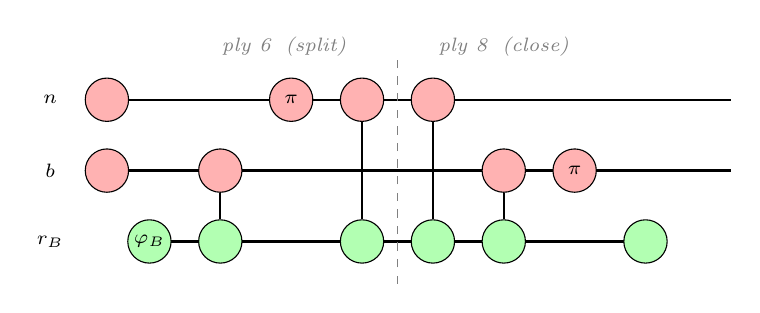
\begin{tikzpicture}[scale=0.9]
  \draw[zxw] (-0.6,2) -- (8.2,2);
  \draw[zxw] (-0.6,1) -- (8.2,1);
  \draw[zxw] (0,0) -- (7,0);
  \node[zxlab] at (-1.4,2) {$n$};
  \node[zxlab] at (-1.4,1) {$b$};
  \node[zxlab] at (-1.4,0) {$r_B$};
  \node[zxx] at (-0.6,2) {};
  \node[zxx] at (-0.6,1) {};
  \node[zxz] (prep) at (0,0) {$\varphi_B$};
  \node[zxz] (g1) at (1,0) {};
  \node[zxx] (x1) at (1,1) {};
  \draw[zxw] (g1) -- (x1);
  \node[zxx] at (2,2) {$\pi$};
  \node[zxz] (g2) at (3,0) {};
  \node[zxx] (x2) at (3,2) {};
  \draw[zxw] (g2) -- (x2);
  \node[zxz] (g3) at (4,0) {};
  \node[zxx] (x3) at (4,2) {};
  \draw[zxw] (g3) -- (x3);
  \node[zxz] (g4) at (5,0) {};
  \node[zxx] (x4) at (5,1) {};
  \draw[zxw] (g4) -- (x4);
  \node[zxx] at (6,1) {$\pi$};
  \node[zxz] at (7,0) {};
  \draw[dashed, gray] (3.5,-0.6) -- (3.5,2.6);
  \node[zxlab, gray] at (1.9,2.75) {ply 6 \;(split)};
  \node[zxlab, gray] at (5.0,2.75) {ply 8 \;(close)};
\end{tikzpicture}
\end{center}

White's diamond is the same diagram on $d$, $c$, $r_W$ with phase $\varphi_W$,
and is disconnected from it.

\paragraph{The reduction.}
All green spiders sit on the $r_B$ wire and are connected along it, so they fuse
into one with phase $\varphi_B$ and four legs; all red spiders on $n$ fuse, with
phases adding to $\pi$, and likewise on $b$:

\begin{center}
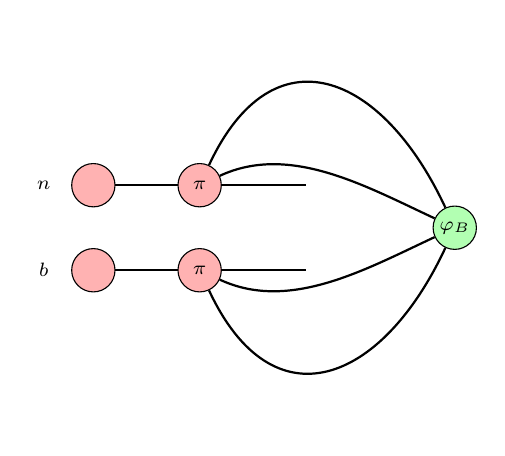
\begin{tikzpicture}[scale=0.9]
  \draw[zxw] (-0.8,2.4) -- (2.2,2.4);
  \draw[zxw] (-0.8,1.2) -- (2.2,1.2);
  \node[zxlab] at (-1.5,2.4) {$n$};
  \node[zxlab] at (-1.5,1.2) {$b$};
  \node[zxx] at (-0.8,2.4) {};
  \node[zxx] at (-0.8,1.2) {};
  \node[zxx] (xn) at (0.7,2.4) {$\pi$};
  \node[zxx] (xb) at (0.7,1.2) {$\pi$};
  \node[zxz] (g) at (4.3,1.8) {$\varphi_B$};
  \draw[zxw] (g) to[out=155,in=25,looseness=0.9] (xn);
  \draw[zxw] (g) to[out=115,in=65,looseness=1.6] (xn);
  \draw[zxw] (g) to[out=205,in=335,looseness=0.9] (xb);
  \draw[zxw] (g) to[out=245,in=295,looseness=1.6] (xb);
\end{tikzpicture}
\end{center}

The green spider is joined to each red spider by exactly two edges. By the Hopf
law each pair disconnects, leaving

\begin{center}
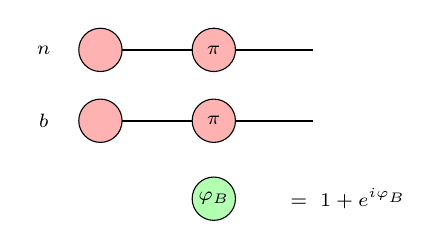
\begin{tikzpicture}[scale=0.9]
  \draw[zxw] (-0.6,2) -- (2.4,2);
  \draw[zxw] (-0.6,1) -- (2.4,1);
  \node[zxlab] at (-1.4,2) {$n$};
  \node[zxlab] at (-1.4,1) {$b$};
  \node[zxx] at (-0.6,2) {};
  \node[zxx] at (-0.6,1) {};
  \node[zxx] at (1.0,2) {$\pi$};
  \node[zxx] at (1.0,1) {$\pi$};
  \node[zxz] at (1.0,-0.1) {$\varphi_B$};
  \node[zxlab] at (2.9,-0.1) {$=\;1+e^{i\varphi_B}$};
\end{tikzpicture}
\end{center}

that is: $n$ and $b$ each become $|1\rangle$ unconditionally, and Black's entire
diamond has become a legless green spider, which is the scalar
$1+e^{i\varphi_B}$.

\begin{remark}[Scalars]
We compute scalars by direct evaluation rather than by chasing normalisation
factors through the rewrites; the diagrams display the structure and
Appendix~\ref{app:verif} supplies the numbers. We note this so that no
rewrite-convention is being silently relied on.
\end{remark}

\subsection{The numbers}

Composing the two diamonds,
\[
  \gr{T} = (1+e^{i\varphi_B})(1+e^{i\varphi_W})\,
           \big|\,nbdc = 1111\,\big\rangle ,
\]
so the unsigned amplitude is $4$ --- the path count of
Appendix~\ref{app:trace} --- and a single minus sign on either fork gives $0$,
which is Question~\ref{q:annihilate} in diagrammatic form: the scalar spider
evaluates to zero and the whole diagram with it.

\subsection{The measurement variant}

Replacing ply 8 by $\Meas\ (f6)!(B,\textsf{Knight}(R))$ substitutes a red effect
on the $n$ wire for the closing CNOTs:

\begin{center}
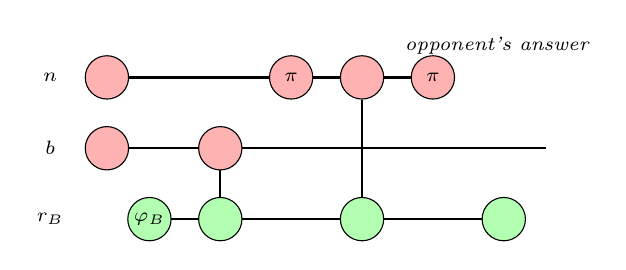
\begin{tikzpicture}[scale=0.9]
  \draw[zxw] (-0.6,2) -- (4.0,2);
  \draw[zxw] (-0.6,1) -- (5.6,1);
  \draw[zxw] (0,0) -- (5.0,0);
  \node[zxlab] at (-1.4,2) {$n$};
  \node[zxlab] at (-1.4,1) {$b$};
  \node[zxlab] at (-1.4,0) {$r_B$};
  \node[zxx] at (-0.6,2) {};
  \node[zxx] at (-0.6,1) {};
  \node[zxz] at (0,0) {$\varphi_B$};
  \node[zxz] (g1) at (1,0) {};
  \node[zxx] (x1) at (1,1) {};
  \draw[zxw] (g1) -- (x1);
  \node[zxx] at (2,2) {$\pi$};
  \node[zxz] (g2) at (3,0) {};
  \node[zxx] (x2) at (3,2) {};
  \draw[zxw] (g2) -- (x2);
  \node[zxx] at (4.0,2) {$\pi$};
  \node[zxlab] at (4.9,2.45) {opponent's answer};
  \node[zxz] at (5.0,0) {};
\end{tikzpicture}
\end{center}

The red $\pi$ effect is $\sqrt2\,\langle 1|$, the projection onto \emph{yes}. It
does not fuse with the green spider on $r_B$, being of opposite colour and
joined by a single edge; and since $n$ is correlated with $r_B$, projecting $n$
pins $r_B$. Closing the branch wire afterwards therefore contributes no fringe.
With both signs positive, \emph{yes} leaves $|1011\rangle$ with amplitude $2$
and \emph{no} leaves $|0111\rangle$ with amplitude $2$; in both cases Black's
diamond is destroyed and the surviving factor of $2$ is White's, which still
closes at ply 9.

The same six-qubit circuit, differing in one gate, gives a two-path fringe or no
fringe, and the difference is whether the branch register was uncomputed or
read.

\subsection{The hardware reading}

Strip the labels from Black's diamond and it is a Mach--Zehnder interferometer:
the branch register is prepared in $|0\rangle+|1\rangle$, acquires a relative
phase, and is closed with $\langle 0|+\langle 1|$, while the configuration
register is the apparatus the two arms pass through, arranged so the arms are
indistinguishable at the output. In gate terms, $H$, then $Z(\varphi_B)$, then
$H$, then read $|0\rangle$.

\begin{principle}
A game trace compiles to one interferometer per Q-move that closes, with the two
arms being two move orders and the configuration register playing the role of
the apparatus. The trace interferes exactly where opening theory transposes.
\end{principle}

For this trace: six qubits, two Hadamards, two phase gates, eight CNOTs and four
$X$ gates.

\subsection{What this does and does not show}

It shows the semantics is implementable and checkable, and it locates the
coherence condition: Proposition~\ref{prop:coherence} turns ``the histories must
agree on everything else'' into ``the filter must be redundant'', checkable per
Q-move against the current support.

It does not show that the general translation is easy. Widths above two need
qudit spiders or a binary encoding, which makes the split a small circuit rather
than one spider. Filters that are \emph{not} redundant are genuine projections,
and a trace containing them is post-selected rather than unitary --- the same
hazard identified in the graded where-clause work, reached here by a different
road. And captures, promotion and castling permute the configuration register in
ways commitment bits cannot express; Cantwell's encoding handles them, at a cost
in qubits this trace was chosen to avoid.

It does not settle whether the game is any good. That remains
Question~\ref{q:m}; the appendix shows only that if the answer is favourable,
the resulting objects are ordinary quantum circuits of a particularly legible
shape.

\section{Verification}
\label{app:verif}

\texttt{zxtrace.py} evaluates the trace twice. The \emph{game} side implements
the amplitude semantics directly: a position is a map from configurations to
amplitudes, a Q-move offers each branch at each realisation, keeps the feasible
pairings, and adds amplitudes on coinciding outcomes; nothing about circuits
appears. The \emph{ZX} side builds the six-qubit state vector, prepares each
branch wire as $|0\rangle + e^{i\varphi}|1\rangle$, applies the controlled
permutations, and closes the branch wires with $\langle 0|+\langle 1|$. The two
are compared for all four sign assignments and both answers to the measurement
variant.

\begin{lstlisting}
signs  Black +1   White +1
  game : |1111> : +4      ZX : |1111> : +4      agree: True
signs  Black +1   White -1
  game : (empty support)  ZX : (empty support)  agree: True
signs  Black -1   White +1
  game : (empty support)  ZX : (empty support)  agree: True
signs  Black -1   White -1
  game : (empty support)  ZX : (empty support)  agree: True

measurement variant, opponent answers YES
  game : |1011> : +2      ZX : |1011> : +2      agree: True
measurement variant, opponent answers NO
  game : |0111> : +2      ZX : |0111> : +2      agree: True

ALL CHECKS PASS
\end{lstlisting}

\begin{thebibliography}{9}

\bibitem{akl2010}
S.~G. Akl.
\newblock Quantum Chess.
\newblock School of Computing, Queen's University.
\newblock \url{https://research.cs.queensu.ca/Parallel/QuantumChess/QuantumChess.html}

\bibitem{burke2020}
K.~Burke, M.~Ferland, S.-H. Teng.
\newblock Quantum Combinatorial Games: Structures and Computational Complexity.
\newblock arXiv:2011.03704, 2020.

\bibitem{burke2021}
K.~Burke, M.~Ferland, S.-H. Teng.
\newblock Transverse Wave: An Impartial Color-Propagation Game Inspired by
Social Influence and Quantum Nim.
\newblock \emph{Integers} 21B (A3), 2021. arXiv:2101.07237.

\bibitem{burke2022}
K.~W. Burke, M.~Ferland, S.-H. Teng.
\newblock Quantum-Inspired Combinatorial Games: Algorithms and Complexity.
\newblock \emph{FUN 2022}, LIPIcs vol.~226, 11:1--11:20.

\bibitem{cantwell2019}
C.~Cantwell.
\newblock Quantum Chess: Developing a Mathematical Framework and Design
Methodology for Creating Quantum Games.
\newblock arXiv:1906.05836, 2019.

\bibitem{cheqqers2025}
Quantum Checkers: The Development and Analysis of a Quantum Combinatorial Game.
\newblock arXiv:2506.05962, 2025.

\bibitem{dorbec2017}
P.~Dorbec, M.~Mhalla.
\newblock Toward Quantum Combinatorial Games.
\newblock \emph{Quantum Physics and Logic (QPL)}, EPTCS 266, 2017, p.~237.
arXiv:1701.02193.

\bibitem{goff2006}
A.~Goff.
\newblock Quantum tic-tac-toe: A teaching metaphor for superposition in quantum
mechanics.
\newblock \emph{American Journal of Physics} 74(11):962--973, 2006.

\bibitem{quantumgo2020}
Quantum Go Machine.
\newblock arXiv:2007.12186, 2020.

\bibitem{scholten2026}
D.~Scholten, B.~Westerbaan, S.~Samardjiska.
\newblock Quantum combinatorial games.
\newblock arXiv:2607.06550, 2026.

\end{thebibliography}

\end{document}
